
\documentclass{article}

% Preamble
\title{Linux Guide}
\author{Aaron Baw}

\usepackage{graphicx}
\usepackage{color}
\usepackage{listings}
\usepackage{hyperref}

\definecolor{grey}{gray}{0.4}
\date{\today}
% END of preamble.

\begin{document}

\maketitle

\tableofcontents

\section{I/O Streams}
Standard streams are a standardized way that different pieces of software and devices can communicate with each other. It serves as a protocol
that developers can use to move data from outputs of software to inputs of other software, in a kind of agnostic manner.

As per the convention there are 3 standard I/O streams, namely \textbf{Standard Input}(stdin), \textbf{Standard Output}(stdout) and \textbf{Standard Error}(stderr).\cite{redirectingIO}

\subsection{I/O Uses in UNIX}
I/O Streams play a fundamental part of the inter-workings of UNIX, particularly when it comes to the use of the shell. As per the UNIX 'conise-and-modular'
philosophy, having an abstracted means of communication between pieces of software forms a crucial role in the interoperability of the operating system.

The result of this system is the ability to connect different pieces of software together to achieve powerful functionality.

By default, when using the shell, the \textbf{stdout} stream tends to be the text output of the shell, whereas the \textbf{stdin} stream tends
to be the input from the keyboard, terminated by the enter key on most occassions.

\subsection{I/O Redirection}
One of the many advantages of using Standard Streams is the ability to manipulate the data destinations and origins using some of the in-built tools and commands
provided by UNIX.

An example of this would be through the use of pipe \textbf{$\vert$}, a powerful redirection command.

The pipe command allows the stdout of one command to be redirected to the stdin of another command, instead of the default text output stdout of the terminal, for instance.

\begin{figure}[h]
    \label{Using the Pipe Command}
    \textcolor{grey}{
      \texttt{cat textDocument.txt $\vert$ grep ``john''}
    }
    \caption{An example of stdin/stdout redirection with the pipe command.}
\end{figure}

The greater than symbol \textbf{\textgreater} can also be used to redirect the stdout of a command to write a file rather than display on the terminal output.

\begin{figure}[h]
    \label{Redirecting stdout to write files}
    \textcolor{grey}{
      \texttt{echo "A message" > message.txt}
    }
    \caption{An example of stdin/stdout redirection with the \textbf{\textgreater} command.}
\end{figure}

Below is a summary of some of the useful commands that can be used to redirect Standard Streams:

      \begin{itemize}
        \item $\vert$ : Pipe. Used to redirect stdout of one command into the stdin of another.
        \item \textgreater : Used to redirect stdout of a command to be written to a specified file.
        \item \textgreater\textgreater : Same as \textgreater but instead appends to the beginning of the file if a file already exists.
        \item \textless : Used to read a file and send this as the stdin of a commnad.
      \end{itemize}

These commands are very versatile, and are able to operate with each other to achieve a wide scope of functionality. Furthermore, they can
also be nested within each other.

\begin{figure}[h]
    \label{Nesting and combining Standard I/O commands}
    \textcolor{grey}{
      \texttt{cat data.txt | sort -n | sed -n 1,1p | column -t > processedData.txt}
    }
    \caption{Combining and nesting I/O redirection commands.}
\end{figure}

In the example above a text file is being read, and then piped into the \textbf{sort} command, of which the output of this command is then piped into
\textbf{sed} where the first row is being selected, and finally this output is then sent to \textbf{column} which organizes the output into a column. After
the data has been processed, the \textbf{\textgreater} command writes the final output from the \textbf{column} command to a file \textbf{`processedData.txt'}.

\section{Linux Filesystem Permissions}

\subsection{Understanding the permissions system on linux}
The permissions for a given file or directory in linux can be viewed with the \textbf{ls -l} command.

  \begin{figure}[h]
    \label{perm1}
    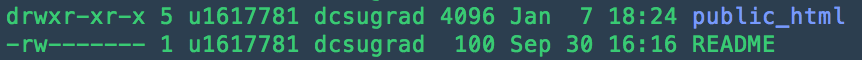
\includegraphics[width=100mm]{/dcs/16/u1617781/public_html/CS133/assignment/permissionsListing.png}
    \caption{Sample output for the \textbf{ls -l} command illustrating linux file permissions.}
  \end{figure}\cite{permScreenshot1}

As you can see above, the permissions for each file is listed in the left-most column of the command output. There are four key components to the permissions layout:

\begin{figure}[h]
  \begin{itemize}
    \item Each portion of the permissions string represents a different feature. The first character states if the item is a file (denoted by \textbf{-}),
    a directory (denoted by \textbf{d}), or a symbolic link (denoted by \textbf{l})
    \item The rest of the permissions string states the level of access each entity on the system has to that particular file. Out of the next 9 characters,
    the first 3 represent the permissions for the owner of the file (typically the creator), then the next 3 characters represent the permissions for the user group, and finally
    the last 3 characters represent the permissions for all users.
    \item Each subsection of 3 characters as outlined above use the same system to illustrate the level of permissions a particular system entity has for the file.
    The presence of \textbf{r} means that the entity can read the file, \textbf{w} means that the entity can write to the file, and finally \textbf{x} means that the entity
    can execute the file. Where a \textbf{-} character is used in place of what would otherwise be a \textbf{r,w or x}, it means that this particular permission is omitted
    from the entity.
  \end{itemize}
\end{figure}

\subsection{Changing permissions on linux}
A popular way of altering the permissions on the linux filesystem is to use the \textbf{chmod} command.

There are a number of different ways that this can be used. Firstly, the perhaps clearest way to alter commands of a particular file is through the following general syntax:

\begin{figure}[h]
    \label{perms2}
    \textcolor{grey}{
      \texttt{chmod a+x filename}
    }
    \caption{Simple alteration of filesystem permissions on linux with the \textbf{chmod} command.}
\end{figure}

Of the first argument passed to the command (\textbf{a+x}), where the \textbf{`a'} character is positioned stands for the entity that is being targeted.
The \textbf{`a'} character stands for `all users'. Other options include \textbf{`o'} (file owner) and \textbf(`g') (user group).

Where the \textbf{`+'} lies indicates whether the following specified permissions should be added (indicated by the \textbf{+} in this instance), or removed,
(which would be denoted by the presence of a \textbf{-} symbol), from the preceeding system entity.

Finally, the last symbol position, in this example the \textbf{`x'} character, indicates what permissions should be altered (in this case added). In this instance,
the \textbf{x} character stands for `eXecute' as may be implied. Other options include \textbf{r} (read) and \textbf{w} (write).

Overall, the semantic meaning of the example chmod usage above would be to ``add execute permissions for all users on the system.''

The equation below summarizes the funcionality of this particular usage of the \textbf{chmod} command:

\begin{figure}[h]
\begin{equation}
  chmod \quad a/o/g \pm r/w/x \quad filename
\end{equation}
\end{figure}

\subsubsection{Using numerical values to assign permissions}
In linux, filesystem permissions can also be represented by numerical values. For example, a permissions value of \textbf{755} would mean
`rwxr-xr-x' in permissions-string form. Much like earlier, each numberical position represents the permissions that each corresponding entity would have;
in the same owner-usergroup-allusers order that was outlined earlier.

Each permission \textbf{r, w or x} has a specific numerical value as can be seen in figure 6.\cite{permValues}

\begin{figure}[h]
  \label{perms3}
  \begin{itemize}
    \item \textbf{r}: 4
    \item \textbf{w}: 2
    \item \textbf{x}: 1
  \end{itemize}
  \caption{Permission numerical values.}
\end{figure}

The individual values of each of the permissions can be added together to form the permissions for each system entity. For example,
if you were to only desire read and execute capability for a particular file, you would only need to add up the corresponding values,
in this case being \textbf{5}. If you desired all other entities to have the same permissions, then the total permission value would be \textbf{555}.

Finally, this permission value can be appled to any file just as one would expect with the \textbf{chmod} command.

\begin{figure}[h]
  \label{perms4}
  \textcolor{grey}{
    \texttt{chmod 555 filename}
  }
  \caption{Assigning permissions directly with chmod.}
\end{figure}

\section{Bash Scripting}
Bash scripting forms a major part of the linux operating system experience. The interoperability of modular commands and standard streams means
that combining commands to produce new functionality becomes quite intuitive.

\subsection{Declaring variables in Bash}

Variables in bash are loosely-typed meaning that variable types are not
specified. Below is an example of a variable declaration in bash:

\begin{figure}[h]
  \label{bash1}
    \lstset{language=Bash}
    \begin{lstlisting}
        text=``A message goes here''
        sentence=``$text and is used here''

    \end{lstlisting}
    \caption{An example of variable declaration and usage.}
\end{figure}

As you can see above, variables are used with the \textbf{\$} prefix before the variable name. This is a requirement anytime the
value of a variable is desired to be used.

\subsection{Whitespace in Bash}

Something important to note about programming in bash is the significance of \textbf{whitespace}. With the exception of a few programming languages
like \textbf{Python}, for example, most programming languages are fairly agnostic about whitespace. This is not the case in bash.

When declaring variables for instance, there must not be any whitespace between the name of the variable, the equals (\textbf{=}) sign, and the variable
value itself.

Another prevalent example of the importance of keeping whitespace in mind is with the usage of \textbf{IF} statements and \textbf{FOR} loops, for example.

When declaring an \textbf{IF} statement, it is crucial that when using the \textbf{[[ ]]} (double bracket) evaluation, that exactly \textbf{one} space is
present between each portion of the comparison.

When declaring \textbf{IF} statements for example, succeeding the comparison requires a newline and the word \textbf{`then'}, after which
another newline is inserted and the conditional logic of the \textbf{IF} statement can be applied. Without the presence of these newlines, semicolons are required
to tell the interpreter where a newline would otherwise be.

\subsection{IF Statements in Bash}

As mentioned above, whitespace is something important to keep in mind when constructing IF statements in Bash.

Unlike other programming languages which typically evaluate the truthfullness of a statement, in Bash all that is conditional to run a following piece of code is the
\textbf{exit status} of the statement. With a successful exit status, the conditional code block will then execute, otherwise it will not.

To use IF statements in a more traditional manner, it is possible to utilize \textbf{[ ]} syntax after the \textbf{IF} declaration. The
code placed within the brackets (keeping in mind the significance of whitespace as outlined previously) is evaluated much like if it were
forming part of the arguments to the \textbf{test} command.

As such it is possible to run code if a certain value is greater than another value, for example:

\begin{figure}[h]
  \label{bash2}
    \lstset{language=Bash}
    \begin{lstlisting}
      if [ ``$var1'' -gt ``$var2'' ]
      then
        # Do something
      fi
    \end{lstlisting}
    \caption{Declaring an IF Statement in Bash}
\end{figure}

There is also a more traditional syntax that can be used to declare the conditions for IF statements within bash using a double square bracket (\textbf{[[ ]]}) as
opposed to just a single one.

\begin{figure}[h]
  \label{bash3}
  \lstset{language=bash}
  \begin{lstlisting}
    if [[ $var1 > $var2 ]]
    then
      # Do something
    fi
  \end{lstlisting}
  \caption{Declaring an IF Statement in Bash with more familiar syntax.}
\end{figure}

It is still important to note the necessity of a single whitespace between each portion of the statement, particularly between the variable names and the brackets, as well as in between everything else.

\subsection{FOR Loops in Bash}

\textbf{FOR} loops in bash behave quite similarly to that of other familiar programming languages. It is interesting to note that there are some quirky features of bash that allow for some interesting
funcionality.

If, for example, it would be desired to iterate through names from a particular text document, an easy way to do this in Bash would be the following:

\begin{figure}[h]
  \label{bash4}
  \lstset{language=Bash}
  \begin{lstlisting}
    for a in $names
    do
      echo $a # Print out every name for e.g.
    done
  \end{lstlisting}
  \caption{A useful but simple use of \textbf{FOR} in Bash.}
\end{figure}

If it is desirable to loop over a specific set of numbers, then \textbf{seq} can be used, or a more traditional syntax:

\begin{figure}[h]
  \lstset{language=Bash}
  \begin{lstlisting}
    for ((i=0;i<$limit;i++))
    do
      # Do something.
    done
  \end{lstlisting}
  \label{bash5}
  \caption{A more traditional for loop syntax in Bash.}
\end{figure}

FOR loops are particularly useful when used in conjunction with \textbf{arrays} as covered in next chapter.

\subsection{Arrays in Bash}

Arrays operate much in the same way as one would expect in other programming languages. Arrays in Bash can be declared by treating a variable as an array; that is
targeting an element with an index such as for example \textbf{array[\$PositiveInteger]} which would turn the variable `\$array' into an array.
Alternatively, arrays can also be declared using the \textbf{declare -a} command.

\begin{figure}[h]
  \lstset{language=Bash}
  \begin{lstlisting}
    declare -a nameOfArray
  \end{lstlisting}
  \label{bash6}
  \caption{One way to declare an array in Bash.}
\end{figure}

Once arrays have been declared and filled, each element can be accessed with a FOR loop. It is possible to use the \textbf{for a in \$variablename...} syntax for this,
or if index numbers are required, the following syntax can be used:

\begin{figure}[h]
  \lstset{language=Bash}
  \begin{lstlisting}
    for (( i=0; i<$(($array)); i++ ))
    do
      if [[ $i % 2 == 0 ]]
      then
        echo ${array[$i]}
      fi
    done
  \end{lstlisting}
  \label{bash7}
  \caption{Looping through an indexed array in Bash.}
\end{figure}

\subsection{Functions in Bash}

To declare functions in bash, there are a few different types of syntax that can be used, such as:

\begin{figure}[h]
  \lstset{language=Bash}
  \begin{lstlisting}
    function printVariable {
      echo ``Argument passed: $1''
    }
  \end{lstlisting}
  \label{func1}
  \caption{Declaring a function in Bash.}
\end{figure}

Arguments are passed to functions much like arguments are passed to scripts and Bash programs in general, with the syntax \textbf{functionName \$Argument1 \$Argument2 ...} and so on.

Functions do not return values much like in other programming languages, but rather exit codes much like the Bash program as a whole. If
it is required to use the declared function as part of a certain block of code to for example perform some logic, the output of this can be assigned to a variable as follows:

\begin{figure}[h]
  \lstset{language=Bash}
  \begin{lstlisting}
    variable=$(calculate $argument)
  \end{lstlisting}
  \label{func2}
  \caption{Saving the result of a function.}
\end{figure}

The use of the dollar sign and parenthesis \textbf{\$(...)} tells the interpreter to save any stdout of the function to the variable.

\subsection{Variable scope in Bash}

When it comes to defining functions to be used in Bash, something to note is the \textbf{scope} of each of the variables.

Each variable that is declared \textbf{within} a function, can \textbf{only} be used within that function. That is, its scope is only that of its nearest parent code block.

Variables that are declared outside of the scope of any function or code block such as an IF statement or FOR loop have a \textbf{global scope} and can be used within any child code blocks.

The same is true for any variable declaration; child code blocks inherit the variable scope of their parents.

\bibliographystyle{ieeetr}
\bibliography{linuxGuideBibliography}

\end{document}
